\documentclass[dp]{FEIstyle}

% Author of the thesis
\FEIauthor{BC. Marcel Soták}

% Evidence number
\FEIregNr{FEI-16607-111443}

% Title
\FEItitle{Aplikácia na organizovanie stretnutí na základe polohy používateľa}
\FEItitleEn{Application for Organizing Meetings Based on User Location}

% Date
\FEIdate{10}{03}{2026}

% Keywords
\FEIkeywords{záverečná práca, šablóna, \LaTeX, formátovanie textu, citácie}
\FEIkeywordsEn{Final thesis, events, meeting, organizer, location, gps, kotlin, android}

% Further details
\FEIstudyProgramme{Aplikovaná informatika}
\FEIstudyProgrammeEn{Applied Informatics}
\FEIstudyField{Informatika}
\FEIstudyFieldEn{Informatics}
\FEItrainingWorkplace{Ústav informatiky a matematiky (FEI)}
\FEItrainingWorkplaceEn{Institute of Informatics and Mathematics (FEI)}

% Supervisor
\FEIsupervisor{Ing. Maroš Čavojský, PhD.}

% Consultant
% -- if there is none, comment out the next line
%\FEIconsultant{tituly Meno Priezvisko, tituly}

% Glossaries -- terms and abbreviations.
% If you use automatic glossaries,
% uncomment the next line.
%\FEIglossaries{includes/glossary}

% Bibliography database file
\bibliography{includes/bibliography.bib}

% Extra packages
\usepackage{float}
\usepackage{array}
\usepackage{amssymb}

% Farby pre výpisy kódu
\definecolor{codegreen}{rgb}{0,0.6,0}
\definecolor{codegray}{rgb}{0.5,0.5,0.5}
\definecolor{codepurple}{rgb}{0.58,0,0.82}
\definecolor{backcolour}{rgb}{0.95,0.95,0.92}
\definecolor{keywordcolor}{rgb}{0,0,0.7}

\lstdefinestyle{mystyle}{
    backgroundcolor=\color{backcolour},
    commentstyle=\color{codegreen},
    keywordstyle=\color{keywordcolor}\bfseries,
    numberstyle=\tiny\color{codegray},
    stringstyle=\color{codepurple},
    basicstyle=\ttfamily\footnotesize,
    breaklines=true,
    captionpos=b,
    keepspaces=true,
    numbers=left,
    numbersep=5pt,
    showspaces=false,
    showstringspaces=false,
    tabsize=2,
    frame=single
}
\lstset{style=mystyle}

\begin{document}

%%%%%%%%%%%%%%%%%%
%%              %%
%% FRONT MATTER %%
%%              %%
%%%%%%%%%%%%%%%%%%
\frontmatter

\FEIpdfInfo
\FEIcover
\FEItitlePage
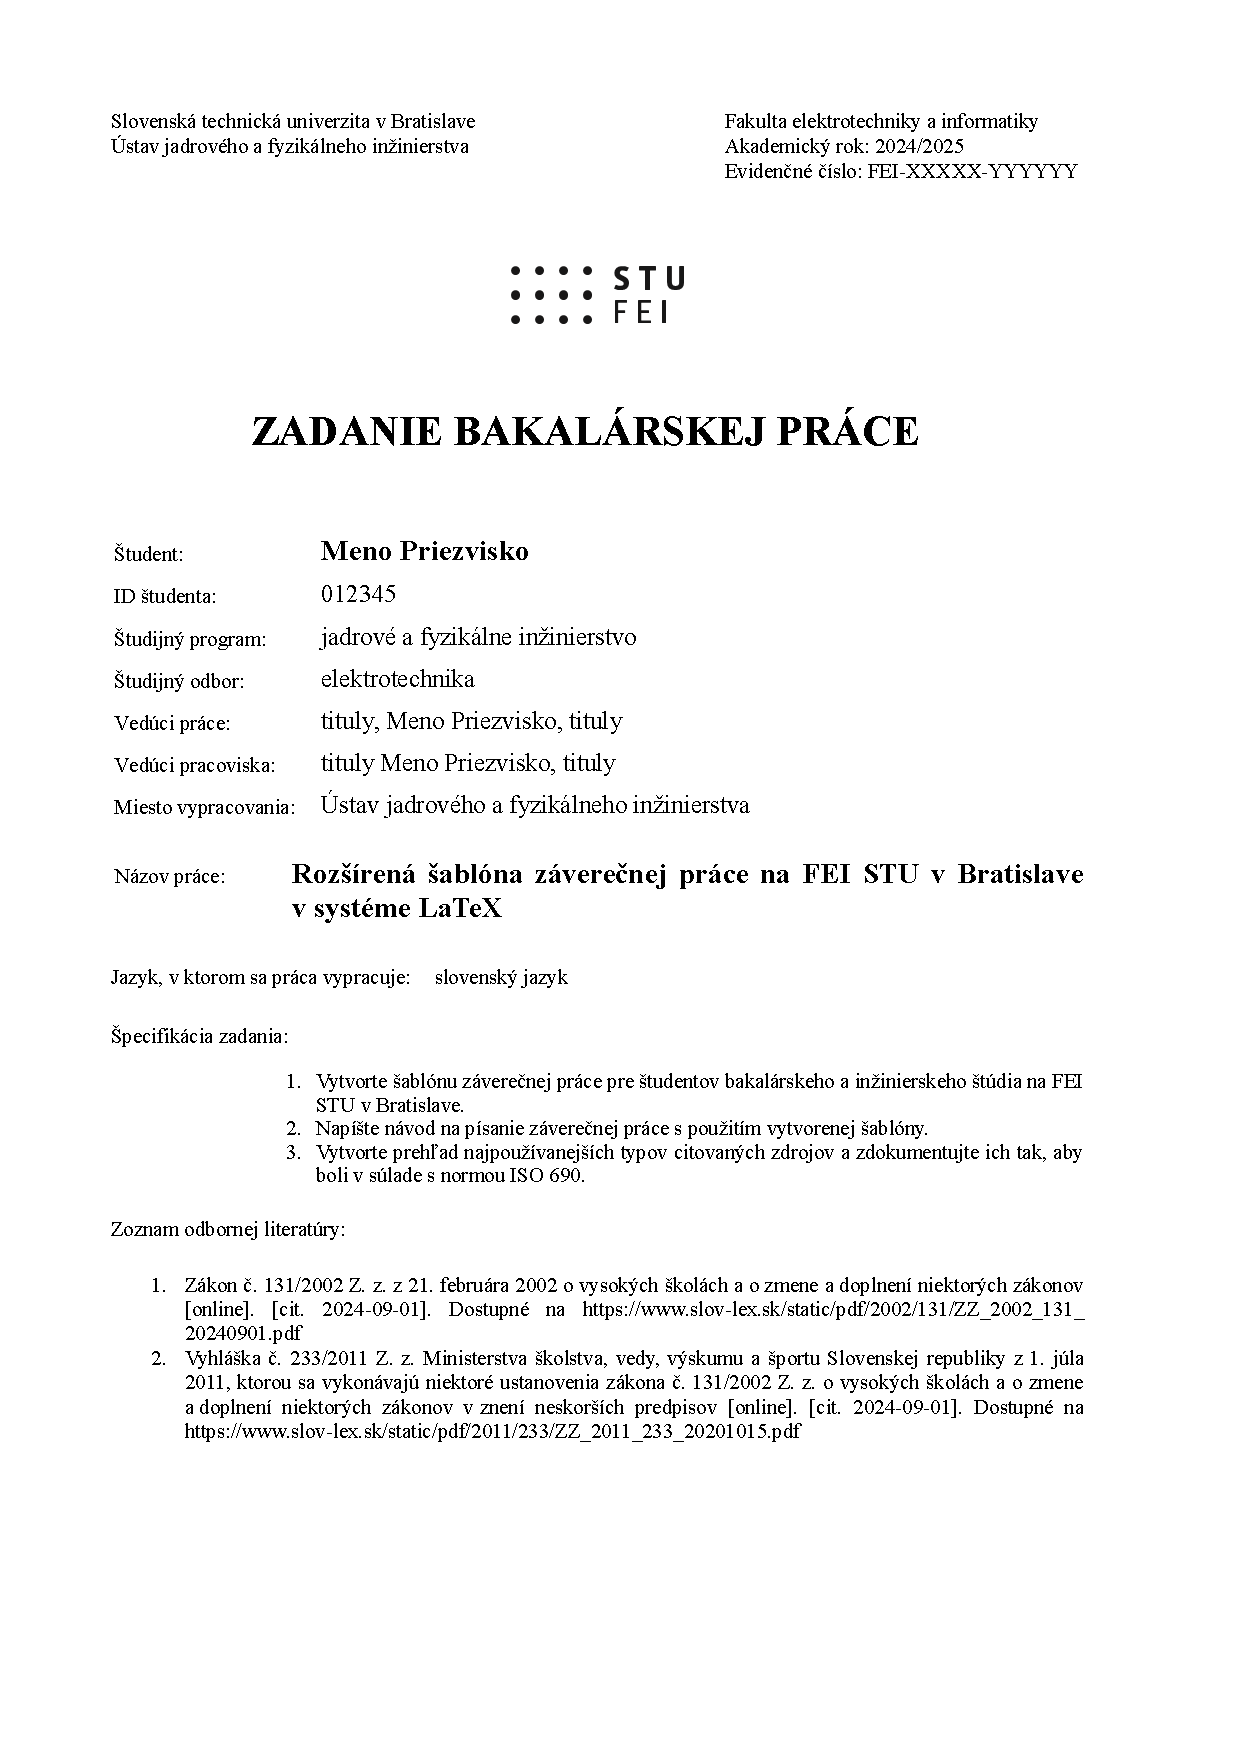
\includepdf[pages=-]{includes/assignment.pdf}
\FEIthanks{includes/thanks}
\FEIabstract{includes/abstract}
\FEIabstractEn{includes/abstractEN}
\FEIcontent
%\FEIlistOfFiguresAndTables

%% List of units and abbreviations
%%
%% Choose the method of typesetting the list of
%% units and abbreviations.
%% Uncomment only one of the two lines below!

%% METHOD 1:
%% ---------
%% Automatically generated and sorted list of
%% abbreviations with hyperlinks from the text.
%% Edit includes/glossary.tex.
%\FEIlistOfGlossaries
%% METHOD 2:
%% ---------
%% Manual list -- must be manually filled and sorted,
%% does not make hyperlinks from the text.
%% Edit includes/manual_glossary.tex.
\FEImanualListOfGlossaries{includes/manual_glossary}

%% Lists of algorithms and listings
\FEIlistOfAlgorithms
\FEIlistOfListings

%%%%%%%%%%%%%%%%%
%%             %%
%% MAIN MATTER %%
%%             %%
%%%%%%%%%%%%%%%%%
\mainmatter

\FEIintroduction{includes/introduction}

\FEIcore{includes/my_core}

%\FEIcore{includes/core}
\FEIconclusion{includes/conclusion}

%% Uncomment only if the document is writen in english
%\FEIresume{includes/resume}

%%%%%%%%%%%%%%%%%%
%%              %%
%% Bibliography %%
%%              %%
%%%%%%%%%%%%%%%%%%
\FEIbibliography
%% AI Declaration
\FEIaiDeclaration{includes/ai_declaration}

%%%%%%%%%%%%%%%%%%
%%              %%
%% BACK MATTER  %%
%%              %%
%%%%%%%%%%%%%%%%%%
\backmatter

%% Attachment A
\FEIappendix{Algoritmus\label{att:algorithms}}{includes/attachmentA}

%% Attachment B
\FEIappendix{Výpis dlhého kódu\label{att:listings}}{includes/attachmentB}

%% Attachment C
\FEIappendix{Slovníček pojmov\label{att:dictionary}}{includes/attachmentC}

%% Attachement D
%\FEIappendix{Súborová štruktúra projektu\label{att:files}}{includes/attachmentD}


\end{document}
